%------------------------------------------------------------------------------
% physor2014_template.tex - template to write a contribution for the PHYSOR 
% 2014 conference
% v1.0 20130422 Wilfred van Rooijen, University of Fukui
%------------------------------------------------------------------------------
% Usage: this template file should be used ONLY with pdfLaTeX. Users who
%        normally use LaTeX need to convert their figures from (E)PS to PDF.
%        See the end of this file for several tips & tricks. Place this 
%        template file and the file physor2014.sty in the same working
%        directory. If you use bibtex, put physor.bst and physor2014.bib also
%        in the working directory. If you have your own BiBTeX database file,
%        make a copy or link in your working directory and replace 
%        \bibliography{physor2014} with \bibliography{your_bib_file}.
%
% NOTE: when running the PHYSOR2014 style file, you may get warnings regarding
%       the versions of several of the style files used in the PHYSOR2014 tem-
%       plate. These are indications that it is time to update you latex in-
%       stallation, but even if you use the older versions, the PHYSOR2014 tem-
%       plate should work correctly. 
%------------------------------------------------------------------------------
\documentclass[12pt]{article}
%
% NOTE: use \documentclass[12pt,draft]{article} for your initial work. This 
%       will give you the "draft" mode:
%       - a black marker is printed for each "overfull hbox"
%       - figures are not included (only the BoundingBox is indicated)
%       - hyperref is switched off
%
% When your manuscript has "overfull" or "underfull" boxes (see latex output)
% then that means that LaTeX cannot perform a proper line breaking. You can try
% to solve the problem by:
% - adding hyphenation locations in long words: hy\-phe\-na\-tion
% - rewrite the sentence
% - adding space, e.g. "Author \cite{foo}" instead of "Author\cite{foo}"
% Try to get rid of all the underfull and overfull boxes (but sometimes a small
% amount of overfull cannot be avoided). 
%
\usepackage{physor2014}
%
% The basic style file loads a minimum of style files. If you need special 
% styles, simply include them here. For example, you may be interested in the
% following packages.
%
% For anything that involves mathematics, equations, etc
\usepackage{amsmath}
%
% To include figures in your paper. Note the following: manuscripts must be
% prepared in PDF. To do this, use pdflatex to produce PDF directly. pdflatex
% can include figures in the following formats: PDF, JPG, and PNG. For bitmap-
% ped images (photos etc), JPG is the preferred format, because JPG images can 
% be compressed very well in PDF, giving very small PDF files. For graphs and 
% schematics, vector images should be used; these can be either PostScript or
% PDF. If you have your figures as (e)ps, then see the notes at the end of this
% file for how to convert (e)ps to pdf.
%
% Making PDF images with Excel: see
% http://office.microsoft.com/en-us/word-help/convert-a-document-to-pdf-HA102850064.aspx?CTT=1
% To make very pretty drawings with LaTeX, check out PGF/TikZ
%
\usepackage{graphicx}
%
% If you use a table, check out this package. It creates tables with a little
% bit more space around the table entries. The result is a table that is easier
% to read, especially if you have mathematical super/subscripts in your work.
% Also check the manual of the package booktabs because it has some good tips 
% on how to make beautiful and informative tables.
\usepackage{booktabs}
%
% The following package takes care of setting SI units. Simply type 
% \degreeCelsius instead of $^\circ$ C. Also takes care of exponents and powers 
% of ten, as well as lining out numbers on the decimal point if required
% \usepackage{siunitx}
%------------------------------------------------------------------------------

%------------------------------------------------------------------------------
% Define title. Use all CAPITALS.
%------------------------------------------------------------------------------
\title{THIS IS THE TEMPLATE TO WRITE A MANUSCRIPT FOR PHYSOR~2014 WITH \LaTeX, THE TITLE SHOULD NOT EXCEED THREE LINES.}
%
% ...and authors
%
\author{ 
  \textbf{First A. Author and Second B. Author\footnote{You can use foot notes if needed, for instance to include the address of your homepage: \href{http://www.nce.upalookaville.edu/}{www.nce.upalookaville.edu}}} \\
  Department of Nuclear \& Chemical Engineering \\
  University of Palookaville, Palookaville, New Jersey, USA\\
  \href{mailto:f.a.author@upalookaville.edu}{f.a.author@upalookaville.edu}\\
  \href{mailto:s.b.author@upalookaville.edu}{s.b.author@upalookaville.edu}\\
  \\                       % Put an extra empty line for different affiliations 
  \textbf{Third Author\footnote{\href{http://www.harahira.co.jp/ned/}{www.harahira.co.jp/ned/}}} \\
  Nuclear Engineering Division \\
  Harahira Heavy Industry, Mihama, Fukui, Japan\\
  \href{mailto:author.third@harahira.co.jp}{author.third@harahira.co.jp}
}

%------------------------------------------------------------------------------
% The \shortauthor is printed on top of the even pages, and the \shorttitle
% is printed on top of the odd pages.
% Suggested format:
% - One author             : A. Author
% - Two authors            : A. Author \& B. Author
% - Three authors          : A. Author, B. Author \& C. Author
% - More than three authors: A. Author~et~al.
% If the title of your manuscript is very long, then make a short title such
% that it fits on one in the header of the odd pages.
%------------------------------------------------------------------------------
\renewcommand{\shortauthor}      % Author's names here
           {Authors' names, use~et~al.~if more than 3}  
\renewcommand{\shorttitle}       % Short title here
           {Paper Title (shortened version to fit in a single line)}  

%------------------------------------------------------------------------------
% Setup PDF info. This sets several values which are listed as the "properties"
% of the PDF file.
%------------------------------------------------------------------------------
\hypersetup{
  pdftitle=\shorttitle,
  pdfauthor=\shortauthor
}

%------------------------------------------------------------------------------
% Begin document
% You can use \doublespacing for your personal draft. This option will increase
% the line spacing, making it easier to add written comments etc. Be sure to
% switch it off when you make the final version!
% The command \linenumbers switches on line numbers, which are practical when
% reviewing a manuscript. Switch off line numbers when you make your final
% version. 
%------------------------------------------------------------------------------
\begin{document}

%\doublespacing

%\linenumbers

%------------------------------------------------------------------------------
% Make the titlepage and set the pagestyle to fancy throughout
%------------------------------------------------------------------------------
\maketitle

\begin{abstract}
  Provide an informative abstract of about 200 - 250 words. The abstract should give a short overview of all material to be discussed in the paper, including the background and / or justification of the research, the research method(s), the main result(s) and the conclusion(s). From the information in the abstract the reader should be able to determine whether or not the paper (and the presentation) will be worthwhile to study.
\end{abstract}

\keywords{Provide at 3 keywords minimum, 6 keywords maximum}

%------------------------------------------------------------------------------
%
%------------------------------------------------------------------------------
\section{INTRODUCTION}
\label{sect::intro}

Section headers should be all capitals (upper case). The format to enter a personal name is different from country to country. We do not enforce any strict rules. Write your name(s) in a format that feels most natural. If desired, you can emphasize your family name by writing it in ALL CAPITALS. We do not specify specific rules for hyphenation and/or interpunction in names: ``Jean-Marie Leblanc", ``J.-M. Leblanc", or ``Leblanc, JM" are all equally acceptable. If there are two authors with the same affiliation, then use ``Author1 and Author2"; if there are three or more authors with the same affiliation, use ``Author1, Author2, ..., AuthorN, and AuthorN+1".

\emph{Address format:} we do not enforce any specific format. You \emph{must} enter your affiliation. A mail address is \emph{not required}, but may be entered if desired. If you enter your mail address, then give sufficient details, including ZIP code etc. Don't forget the name of the country.

%------------------------------------------------------------------------------
%
%------------------------------------------------------------------------------
\section{SECOND OR SUBSEQUENT MAJOR HEADING}
\label{sect::second}

It is up to the writer to divide the manuscript into sections and sub-sections. For a conference contribution, in general 2 levels of sectioning should be adequate (i.e. sections and sub-sections), but we allow subsub-sections. If you want to make an appendix, check Appendix~\ref{app::a} for details about the format.

%------------------------------------------------------------------------------
%
%------------------------------------------------------------------------------
\subsection{Subsection Title: First Character of Each Non-trivial Word is Uppercase}
\label{subsect::major}

\LaTeX\ has several classes of characters. For instance, there are normal letters, mathematical symbols, and special characters. White space is one of the special characters. In \LaTeX\, a white space does not have a constant width. Rather, the spacing between words is adjusted so that lines and paragraphs are optimally typeset\footnote{In fact, the space between letters in a word is also adjusted to give an optimal paragraph filling. The process of spacing the letters is known as \emph{kerning}.}. A special case is the combination of a period (full stop, ``.") followed by whitespace. This indicates to \LaTeX\ a break between sentences and then it is allowed to stretch space even further. Also, whitespace is interpreted in \LaTeX\ as a potential location for a line break. But sometimes, you want to have some white space, but no line break: for example, when you make a Reference like ``Figure~XYZ``, you want to make sure that a line break does not happen between the ``Figure" and the ``XYZ". In that case, use the special ``unbreakable space" (tilde-sign), i.e. use \verb|Figure~\ref{fig::figure}|. Use this also for citations, i.e. use \verb|See~\cite{book}|. The same applies for the construction ``et~al.", where the space between ``et" and ``al." should be non-stretchable and non-breakable, i.e. \verb|et~al.|. If ``et~al." is used in a running sentence, then use \verb|et~al.~| to make sure that the space after the period is interpreted as a non-stretchable space.

%------------------------------------------------------------------------------
%
%------------------------------------------------------------------------------
\subsubsection{Sub-subsection: use italic font, only first word is capitalized} 
\label{subsubsect::minor}

You can use a sub-subsection if you need to.

%------------------------------------------------------------------------------
%
%------------------------------------------------------------------------------
\section{ANOTHER SECTION: MAKING REFERENCES} 
\label{sect::references}

The \texttt{physor2014} style uses the natbib package to improve the typesetting of references. In general, the normal citation should be sufficient, i.e. \verb|\cite{book}|. However, natbib has various citation commands and allows to put options into the citation command. See the natbib manual for more information. If you want to cite more than one work, simply combine them into one \verb|\cite{}|. The natbib package will make sure that the final typesetting is reasonable, so that you get this: (see~\cite{proc_paper,website,journal,book}); rather than this: (see~\cite{proc_paper},~\cite{website},~\cite{journal},~\cite{book}). References should be listed in the order that they are called out in the text (note: this is automatic if you use Bib\TeX).

%------------------------------------------------------------------------------
%
%------------------------------------------------------------------------------
\subsection{Hyperlinks} 
\label{subsect::hyper}

The \texttt{physor2014} style uses the hyperref package to pretty-print URLs. URLs have no spaces, and are therefore impossible to treat with the normal line breaking algorithms in \LaTeX. Besides, even if a URL is split over a line, then a hyphen-sign should not be inserted. The hyperref package has some more benefits:

\begin{itemize}
\item All references in your document become hyperlinks automatically. When you use a \verb|\ref{}|, the PDF document will have a hyperlink in place which allows you to navigate through your document. This feature is very practical for instance to refer to equations.

\item All bibliographic material is internally linked; one click on the link will show you the book.

\item In the author entry, if used with the \verb|mailto:|-prefix, a hyperlink will be created. If this link is clicked, the default email editor is started and an email to the author is automatically initialized.
\end{itemize}

See the hyperref documentation if you want to know more.

%------------------------------------------------------------------------------
%
%------------------------------------------------------------------------------
\section{EQUATIONS}
\label{sect::equations}

The full power of \LaTeX\ is in typesetting mathematical material. Please use the \texttt{amsmath} package. Note the following: \LaTeX\ provides the \texttt{equation}-environment and the \texttt{equation*}-environment. The starred version produces no equation number. According to tradition, an equation is only given a number if there is a reference to the equation. Indeed, if the equation is not refered to, there is no need for an equation number. But for the present template, strict numbering rules are not enforced. A simple equation:

\begin{equation*}
  a^2 + b^2 = c^2
\end{equation*}

But \LaTeX\ also allows very long equations, such as Equation~\eqref{eq::orig_trans}. Note: please use \verb|\eqref{}| to refer to equations.

\begin{multline}
  \hat \Omega \cdot \nabla \psi ( \vec r, E, \hat \Omega )  + \Sigma_t ( \vec r, E ) \psi ( \vec r, E, \hat \Omega ) = \\ \int \limits_{0}^{\infty} \! \int \limits_{4 \pi} \! \Sigma_s ( \vec r, E^\prime \rightarrow E, \hat \Omega^\prime \rightarrow \hat \Omega ) \psi ( \vec r, E^\prime, \hat \Omega^\prime ) \, \mathrm{d}\hat \Omega^\prime \, \mathrm{d}E^\prime + \\ \frac{\chi ( \vec r, E )}{4\pi} \int \limits_0^\infty \! \int \limits_{4\pi} \nu \Sigma_f ( \vec r, E^\prime ) \psi ( \vec r, E^\prime, \hat \Omega^\prime ) \, \mathrm{d} \hat \Omega^\prime \, \mathrm{d}E^\prime + S_\text{ext} ( \vec r, E, \hat \Omega ) \label{eq::orig_trans}
\end{multline}

Please always introduce all symbols, avoid things like ``all symbols have their normal meaning".

%------------------------------------------------------------------------------
%
%------------------------------------------------------------------------------
\section{FIGURES AND TABLES} 
\label{sect::floats}

\LaTeX\ has many packages to make it easy to include figures into your manuscript. With pdf\LaTeX\, you can include figures as PDF, JPG, or PNG. For bitmapped material, JPG is preferred, because it can be compressed very efficiently into the PDF file and very small PDF files will result. For bitmapped images, please use a resolution of at least 300x300 dpi. For graphs and schematic drawings, please use PDF. This will provide so-called vector-images, which have a very small file size, and which provide optimal resolution under all magnification. To make very nice schematics in pdf\LaTeX\, check out PGF/TikZ. All figures and tables need to be refered to in the running text. Figures or tables without references (``dangling" figures and tables) are not allowed!

One of the issues with \LaTeX\ is that the size of the figure in the final document is not known, and you need several iterations to find the correct size. In general, you can avoid trouble by using the \texttt{[width=]}-option of the \verb|\includegraphics{}| command, in combination with the parameter \verb|\textwidth|. For example, to set two figures side-by-side and remain within the text width, use: 

\begin{verbatim}
  \includegraphics[width=0.45\textwidth]{foo1.pdf}
  \includegraphics[width=0.45\textwidth]{foo2.pdf}
\end{verbatim}

The result would be something like Figure~\ref{fig::sym6}. Obviously, this only works if both figures are roughly equal in size to begin with. See the manual of the graphicx package for more info. If you need to set several figures together, consider the subfigure package which allows to set complex combinations of small figures into one larger figure.

\begin{figure}[ht!]
  \begin{center}
    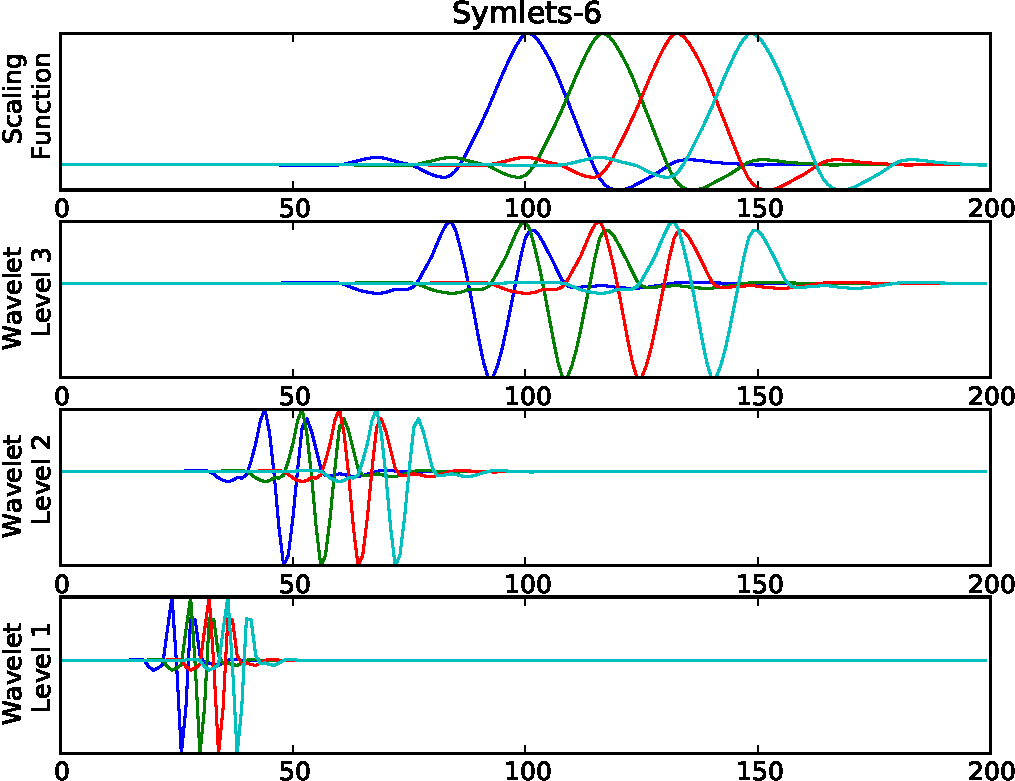
\includegraphics[width=0.45\textwidth]{sym6-crop.pdf}
    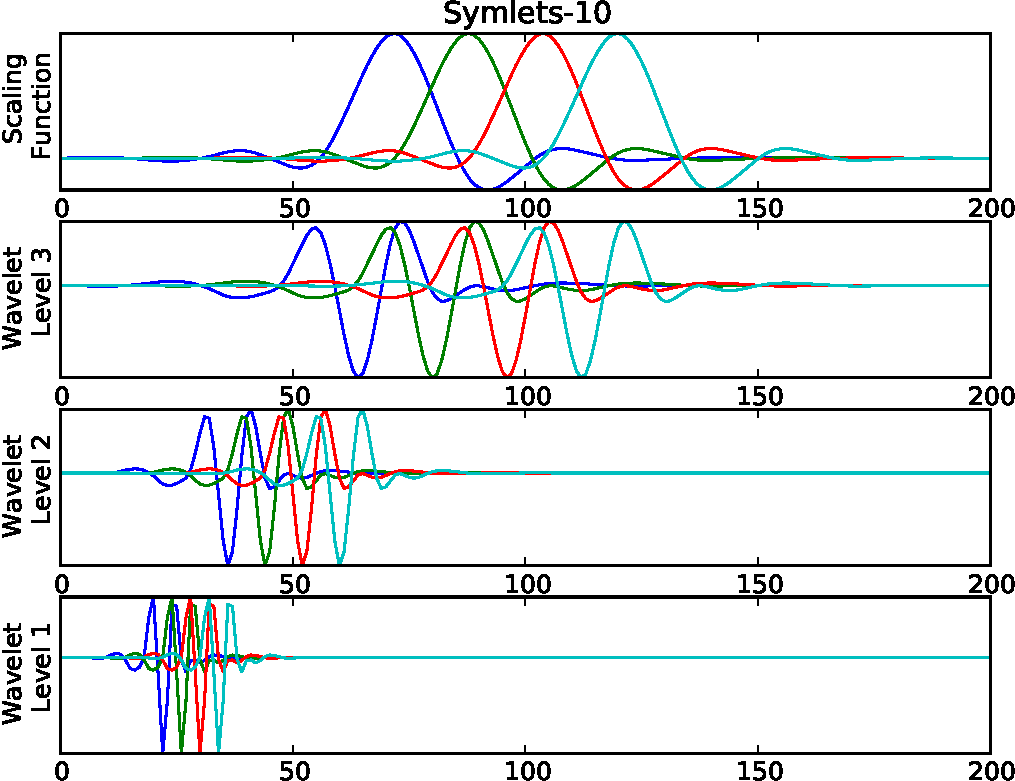
\includegraphics[width=0.45\textwidth]{sym10-crop.pdf}
    \caption[]{\label{fig::sym6}Figure captions go underneath the figure, over the full width of the page.}% Only the ``Figure" label and figure number are bold.}
  \end{center}
\end{figure}

For tables, we do not enforce any special style. Writers are encouraged to take a look at the booktabs package. The manual of this package has some interesting pointers to create beautiful and informative tables. An example of a table is given, see Table~\ref{tab::unc}.

\begin{table}[ht]
  \begin{center}
    \caption{\label{tab::unc}Table captions appear above the table, over the full width of the page. Only the ``Table" label and table number are bold.}
    \begin{tabular}{llll}
    \toprule
    Parameter & \multicolumn{2}{c}{Current uncertainty (LMFBR) [\%]} & Target uncertainty [\%]\\
              & Input data                & Modeling &                    \\
    \midrule
    $k_\text{eff}$          & 1.5 & 0.5 & 0.3 \\
    Power peak              & 1   & 3   & 2   \\
    Power distribution      & 1   & 6   & 3   \\
    Control rod worth       & 5   & 6   & 5   \\
    (element)               &     &     &     \\
    Control rod worth       & 5   & 4   & 2   \\
    (total)                 &     &     &     \\
    Reactivity coefficients & 7   & 15  & 7   \\
    (total)                 &     &     &     \\
    Reactivity coefficients & 20  & 20  & 10  \\
    (component)             &     &     &     \\
    Decay heat              & 10  & 3   & 5   \\
    \bottomrule
    \end{tabular}
  \end{center}
\end{table}

%------------------------------------------------------------------------------
%
%------------------------------------------------------------------------------
\section{CONCLUSION} 
\label{sect::conclusion}

Concluding: good luck with the preparation of your manuscript.

%------------------------------------------------------------------------------
%
%------------------------------------------------------------------------------
\section*{ACKNOWLEDGMENTS}

If you want to thank somebody or something (maybe a funding organisation), do it here.

%------------------------------------------------------------------------------
% Bibliography. There are two ways to include the bibliography in your manu-
% script: 
% 1. use BibTeX: put physor2014.bst in your working directory  -or-
% 2. Manual list of references
% BibTeX is the preferred method, as it will take care of sorting etc automa-
% tically. To use BibTeX you need to make a database (.bib file), see the 
% example in the template. Many programs are available to make a BibTeX data-
% base for you, for example:
% - PyBliographer (http://www.pybliographer.org/)
% - Jabref        (http://jabref.sourceforge.net/)
%
% For BibTeX users: include as many bibliographic details as possible. The 
% physor2014.bst style file will select the relevant fields from your .bib file.
% Most bibliographic data are optional; if a required entry is missing BibTeX
% will complain about it.
% The physor2014.bst file allows the following non-standard options
% - a "doi" field, which will show as http://dx.doi.org/doi_number
% - a "url" field, which will set URLs in the proper way
% - the doi and url fields are processed by hyperref and result in clickable 
%   links
%
% In all cases (both for manual entry and for bibtex): 
% - The authors full name is preferred over initials (i.e. "Mercedes Benz" is 
%   preferred over "M. Benz")
% - List a maximum of three authors, separated by commas. If there are more than
%   threee authors, use "First Author \emph{et al},"
% - List as much bibliographic details as possible but if data are missing then
%   just leave the entries blank
%
% If you use BibTeX: 
\bibliographystyle{physor2014}
\bibliography{physor2014}
%
% If you use manual input, use the following format.
%------------------------------------------------------------------------------
% \begin{thebibliography}{300}
% \bibitem{journal} Some Author(s), ``Article Title,'' \emph{Journal Name}, \textbf{Volume(number)}: pp. 34-89 URL \url{http://dx.doi.org/doi_number} (19xx).
%
% \bibitem{proc_paper} C. D. Author(s), ``Article Title,'' In: \emph{Proceedings of Meeting} (Editor Name, editor), Organisation, Location, Dates of Meeting, Vol. n: pp. 134-156 (19xx).
%
% \bibitem{book} Epsilon F. Author, \emph{Book Title in Italic}, Publisher, City \& Country (19xx). 
%
% \bibitem{website} ``Research Institute of Nuclear Engineering, University of Fukui'', \url{http://www.rine.u-fukui.ac.jp/english/index.html} (2013).
% \end{thebibliography}
%
%------------------------------------------------------------------------------
% Set up for appendices
%------------------------------------------------------------------------------
\appendix

\makeatletter
\def\@seccntformat#1{APPENDIX \csname the#1\endcsname.~}
\makeatother

%------------------------------------------------------------------------------
% If you need to make one (or more) appendix (appendices), place them here as
% sections
%------------------------------------------------------------------------------
\section{HOW TO MAKE APPENDICES}
\label{app::a}

An appendix is a section with extra material which is relevant to the manuscript, but is too bulky, too detailed, or simply too long to include in the main text. Feel free to make one (or more) appendix (appendices), but remember: if you make an appendix, then you must include a reference from the main text to the appendix. An unreferenced (``dangling") appendix is not allowed.

\section{ISSUES RELATED TO FISSION PRODUCT DECOUPLING IN ADJOINT TRANSMUTATION CALCULATIONS}
\label{app::b}

An appendix is a section with extra material which is relevant to the manuscript, but is too bulky, too detailed, or simply too long to include in the main text. Feel free to make one (or more) appendix (appendices), but remember: if you make an appendix, then you must include a reference from the main text to the appendix. An unreferenced (``dangling") appendix is not allowed.

\end{document}

%------------------------------------------------------------------------------
% pdflatex allows figures in PDF, JPG and PNG. For users who have prepared their
% figures in (e)ps, please find here some tips and tricks:
% - Nearly all latex distributions have the tool "ps2pdf". This tool translates 
%   (e)ps files into pdf files, which can be included in pdflatex
% - In some cases, ps2pdf produces a pdf file on a4 size (or US letter size, de-
%   pending on your computer's settings). In such a case, use "pdfcrop" to cut 
%   off the excess white space. Subsequently include the cropped pdf file (by
%   default the file foo.pdf will be renamed foo-crop.pdf). Note: do NOT use
%   foo.crop.pdf! pdflatex will complain that .crop.pdf is not a known graphics
%   format.
% - If you have very many (e)ps files that need conversion, consider making a 
%   BASH script or something similar and use ps2pdf and pdfcrop on each (e)ps
%   file
%------------------------------------------------------------------------------

